\documentclass[12pt]{article}
\usepackage{graphicx}
\usepackage{float}
\usepackage{subfloat}
\begin{document}

\section{Locality of Program Property}

An important assumption of this work is that code fragments generated for dynamic analysis based on a demand can be small. In this section, we further elaborate this assumption and also provide data to support the validity of this assumption. \\

Our initial finding regarding the locality of program properties can be dated back to 2008 [13]. In a demand-driven buffer overflow detection study, we found that for a set of benchmarks we experimented, determining buffer safety is only relevant to statements within 1-4 procedures. \\

\begin{figure}[H]
     \centering
     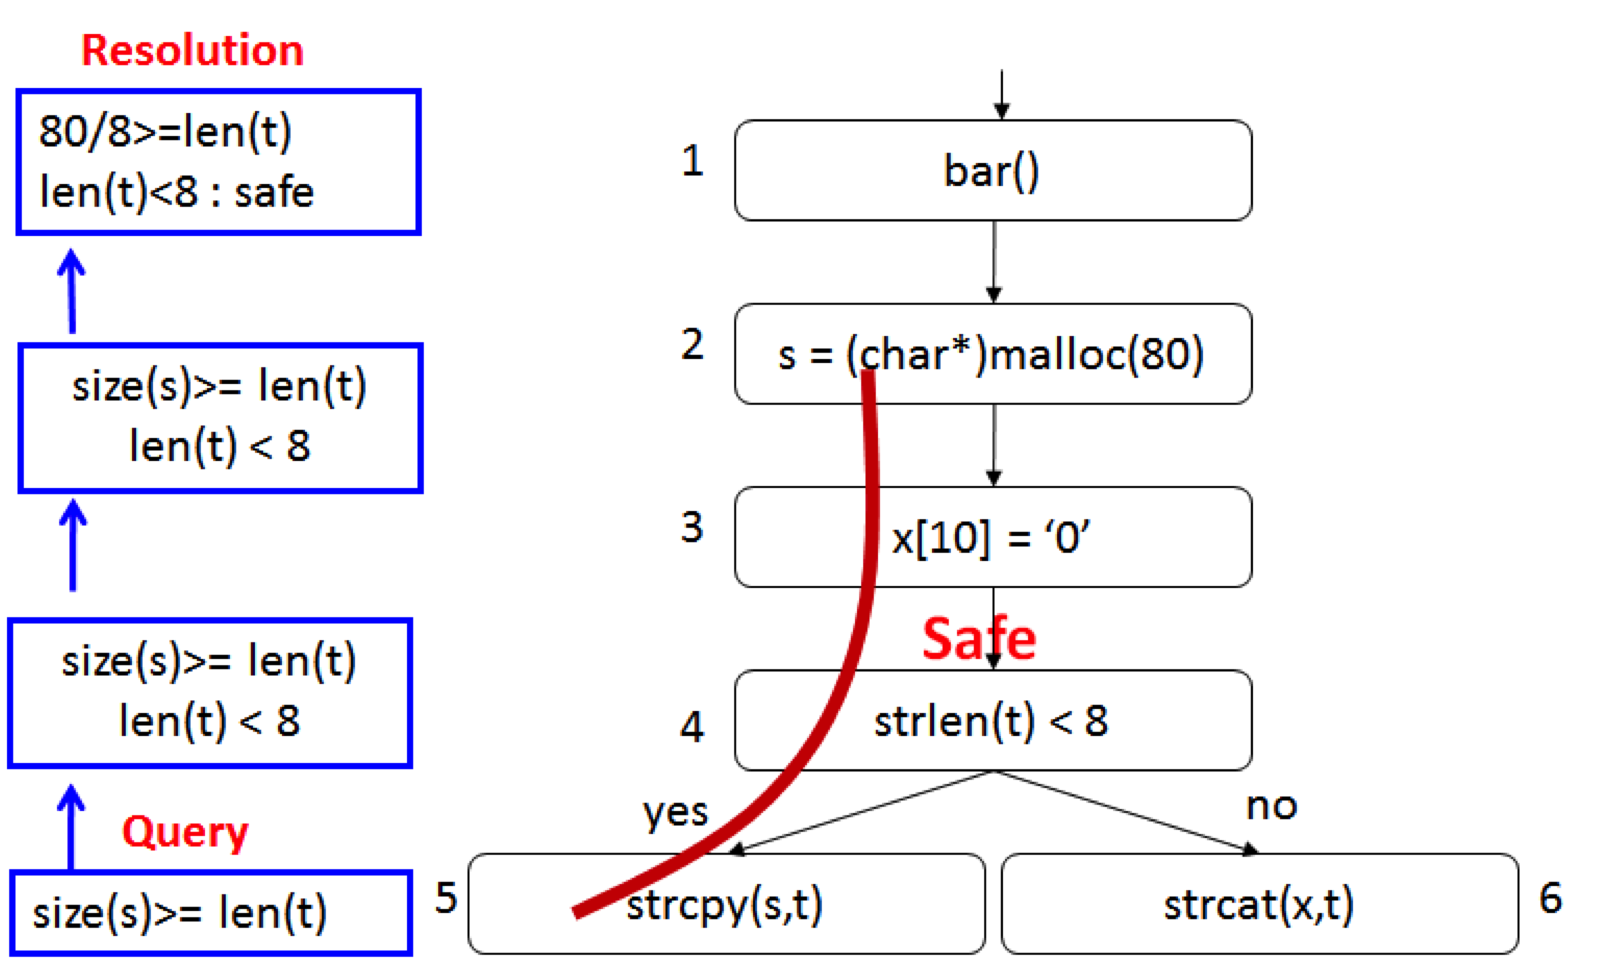
\includegraphics[width=5in]{buffer-overflow-example.png}
     \caption{Localities of Program Properties: Determining Buffer Overflow}
     \label{Buffer Overflow}
 \end{figure}

In Figure 1, we use a simple buffer overflow example to explain. At node 5, the code contains a buffer access. In the demand-driven static analysis, we construct a query $size(s) \geq len(t)$ to inquiry if an overflow can occur. We propagate this query backwards along nodes 2-5, and we are able to determine that the buffer access is safe. It means that for all the paths that reach node 2 and traverse path segment $<2--5>$, the buffer access is safe at node 5. If we construct a code fragment contains nodes 2, 4 and 5, we can determine this program properties.\\

This founding aligns with the psychological implication that developers cannot track many details in their brain. They more likely remember the local context of their code, and the properties of their code should reflect that. We hypothesize that program properties beyond buffer overflow may also manifest such locality. We thus conducted a study in a more general scale.\\

We assembled a set of 50 benchmarks from the top 100 C projects in GitHub and 100 GNU projects. We designed two slice experiments for - 100 randomly selected statements from each benchmark and 50 assert statements from a subset of the benchmarks. We used CodeSurfer to perform backward data slice on these statements. Due to scalability issues and certain build systems being incompatible with CodeSurfer, we selected only projects that were successfully built by CodeSurfer. \\


\begin{figure}[H]
  \centering
  \begin{tabular}{@{}c@{}}
    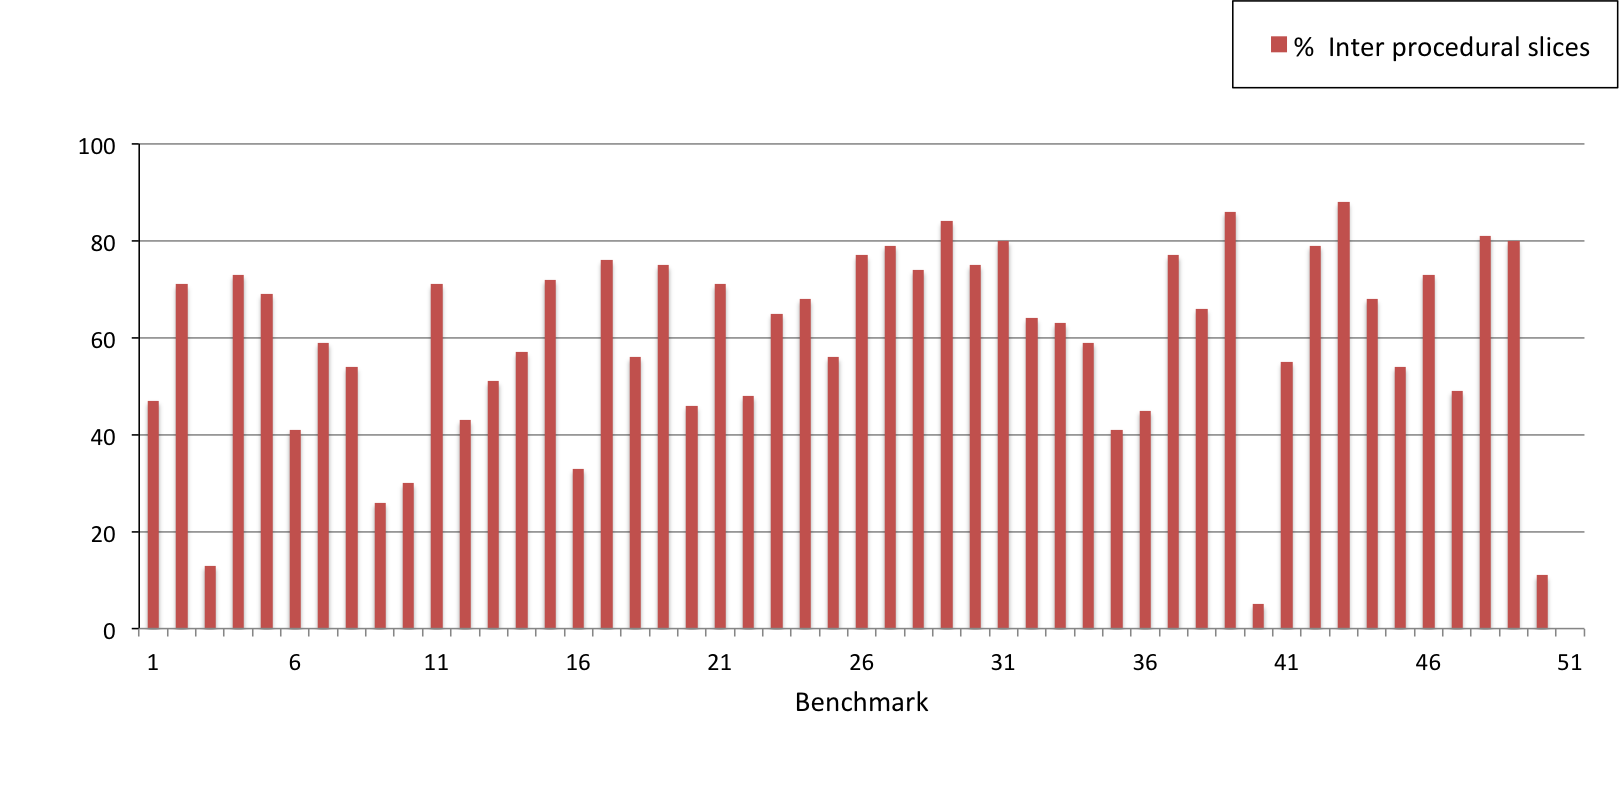
\includegraphics[width=5in]{Inter-procedural-slices.png} \\[\abovecaptionskip]
    \small (a) Random Statements
  \end{tabular}

  \vspace{\floatsep}

  \begin{tabular}{@{}c@{}}
    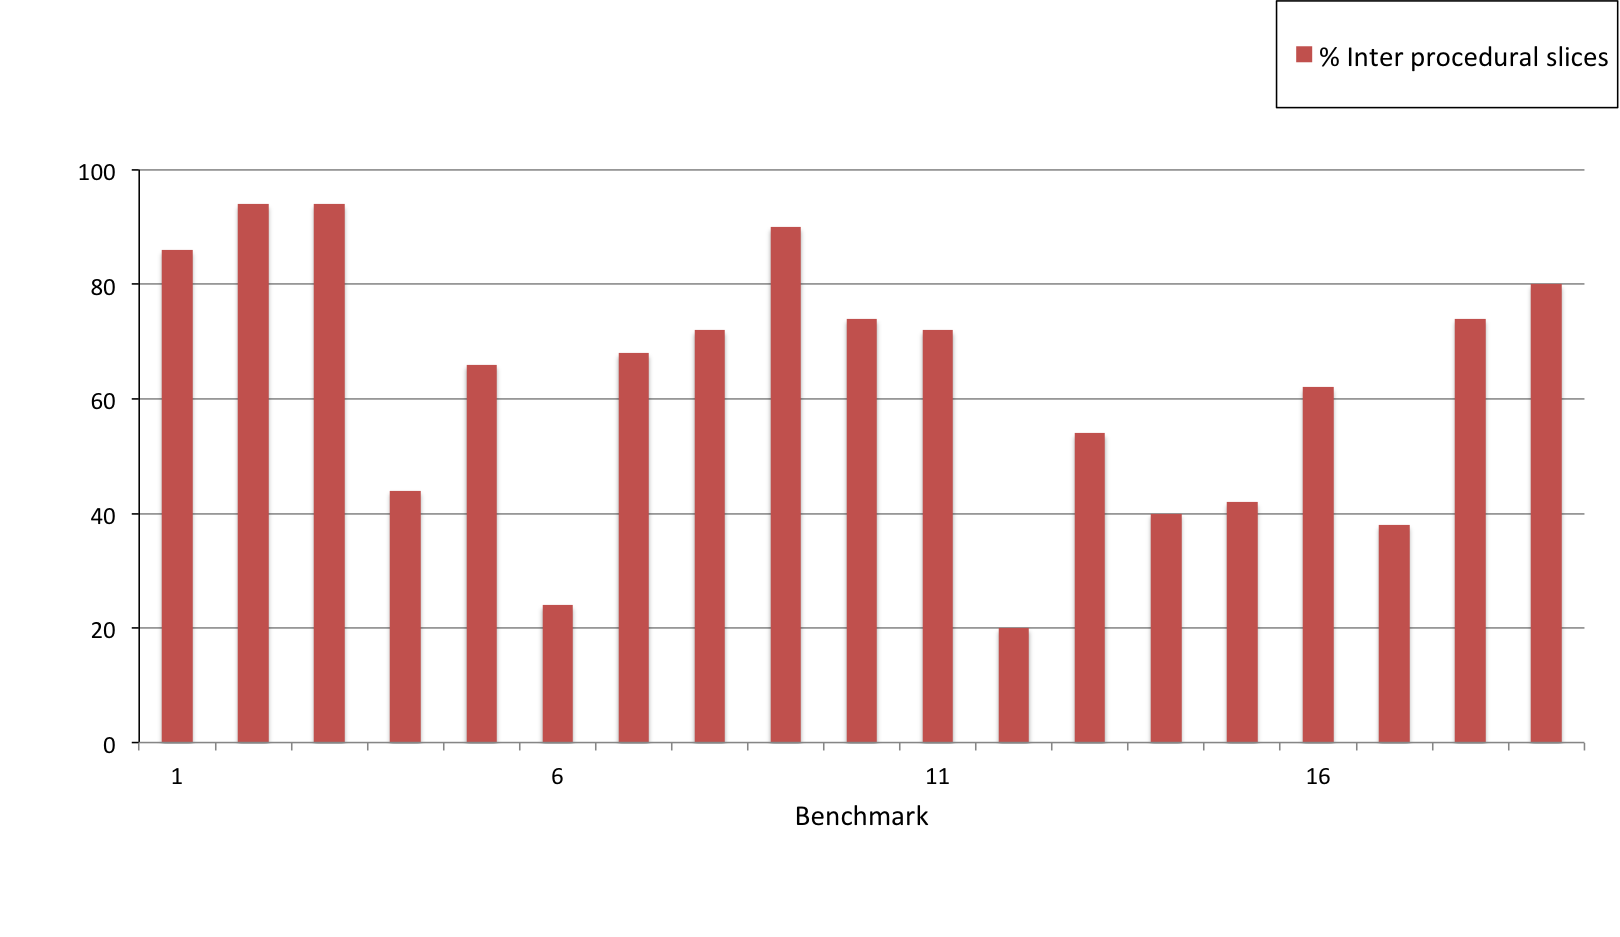
\includegraphics[width=5in]{Inter-procedural-slices-assert.png} \\[\abovecaptionskip]
    \small (b) Assertions
  \end{tabular}
  
  \caption{Slices with Call Sites}\label{slice with call sites}
\end{figure}

We refer to a slice with call sites as an inter procedural slice. To perform analysis of the resultant data slice, we also need to resolve any call sites that are part of the slice. To support this claim, we analyzed the percentage of inter procedural slices for both random statement and assertion experiments. From Figure 2(a) and 2(b), we notice that there are no benchmarks with zero inter-procedural slices. Also, it is evident that more than $85\%$ of benchmarks have at least $40\%$ inter-procedural slices. We also studied number of procedures in slices from a benchmark. The results are shown in Figure 3. \\

\begin{figure}[H]
  \centering
  \begin{tabular}{@{}c@{}}
    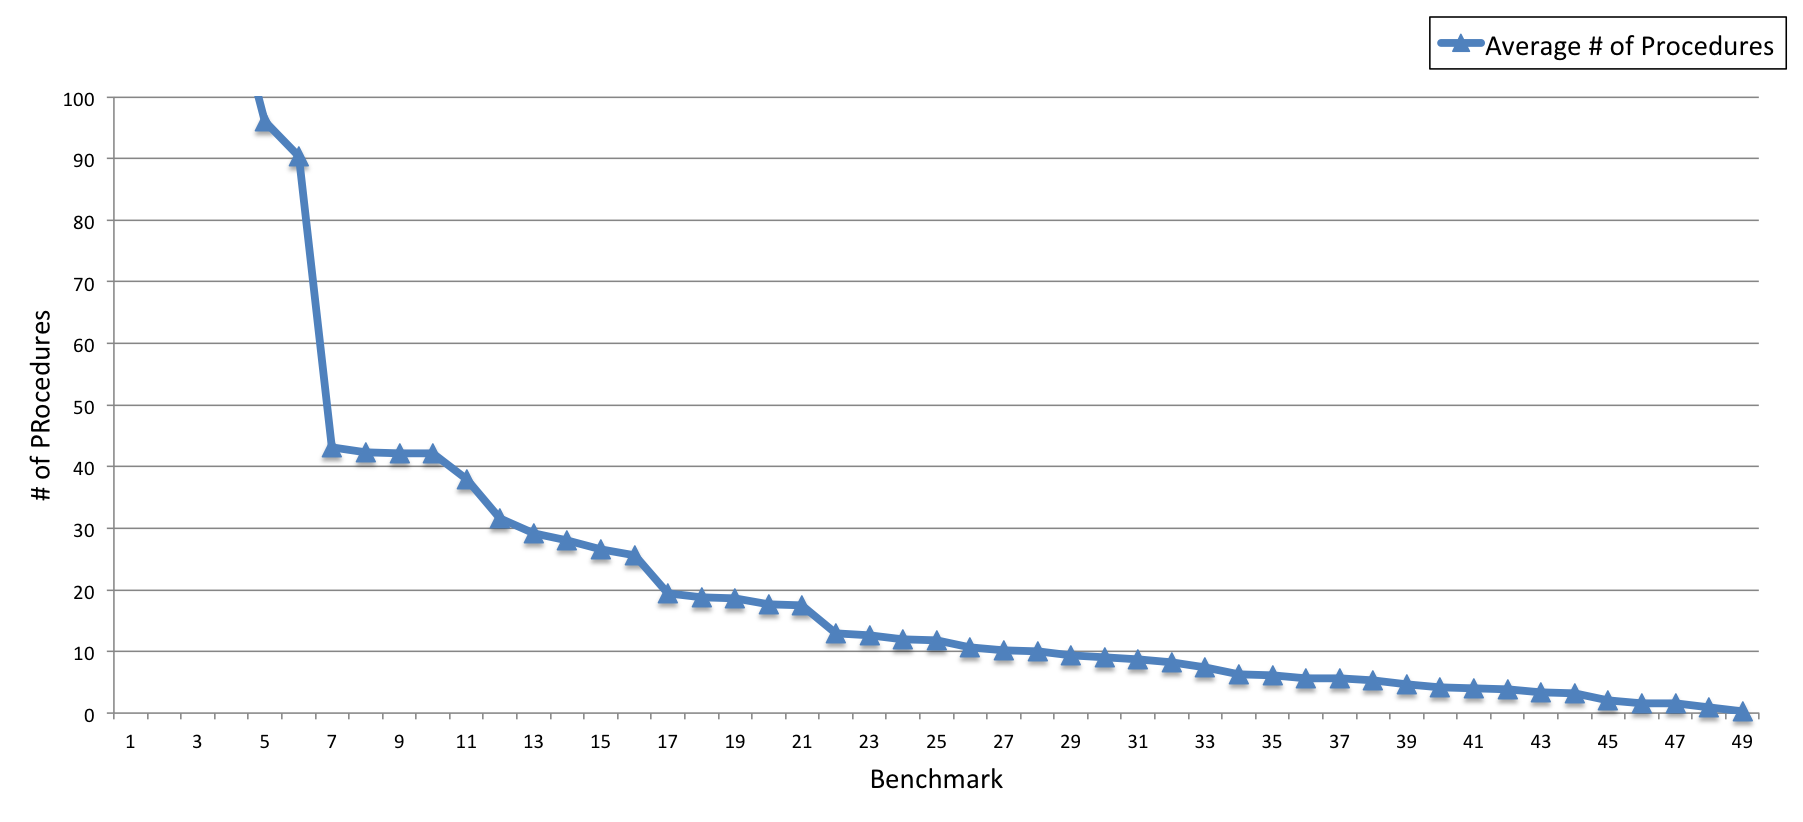
\includegraphics[width=5in]{proc-count.png} \\[\abovecaptionskip]
    \small (a) Random Statements
  \end{tabular}

  \vspace{\floatsep}

  \begin{tabular}{@{}c@{}}
    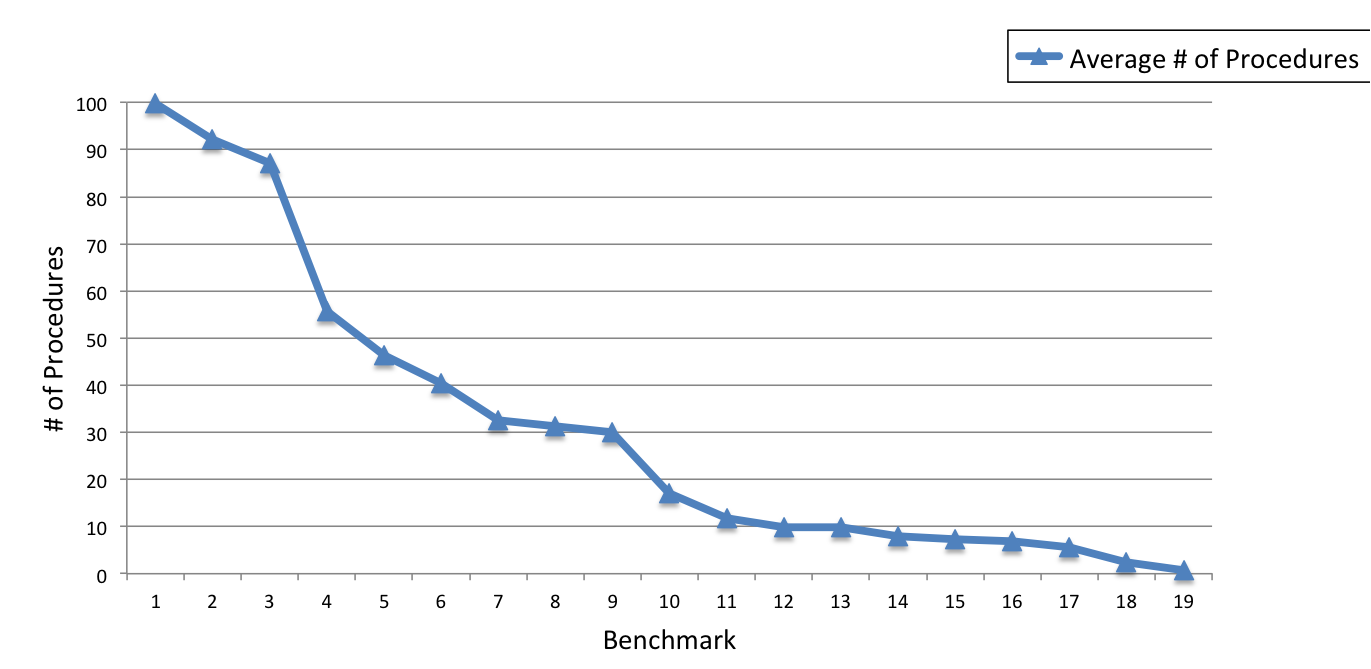
\includegraphics[width=5in]{proc-count-assert.png} \\[\abovecaptionskip]
    \small (b) Assertions
  \end{tabular}
  
  \caption{Average Number of Procedures per Slice}\label{procedure count average}
\end{figure}

Call sites in a data slice are essentially calls to functions that modify variables in the slice. To resolve call sites, we used relevant statements from a full slice of the given statement. A full slice includes control flow, hence all functions that are called from within the data slice are included in the full slice. We now scan the data slice for call sites and for each call site found, we include the statements from the full slice that declare and define the call site. Thus, our approach extracts all statements that influence the variables in the data slice.\\

\begin{figure}[H]
  \centering
  \begin{tabular}{@{}c@{}}
    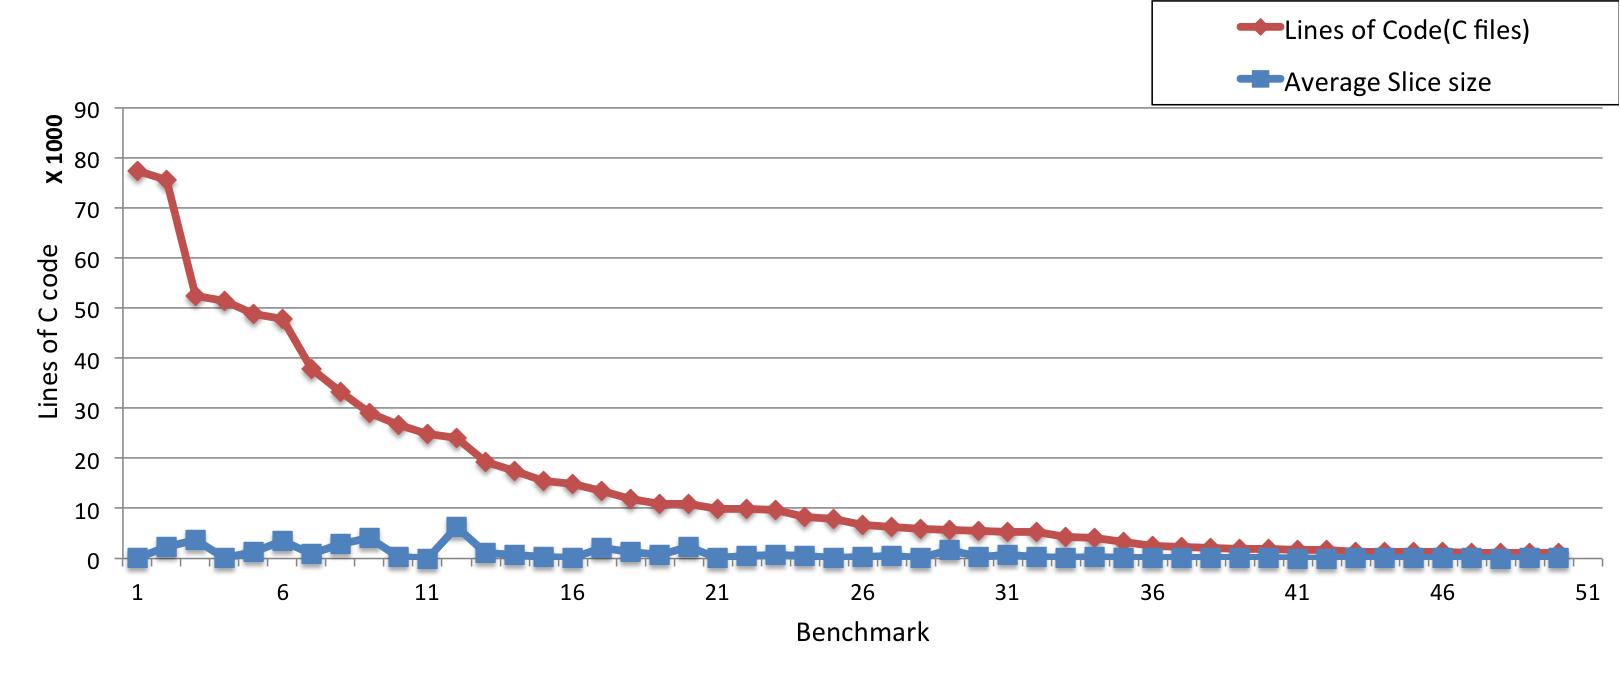
\includegraphics[width=5in]{slice-size-compare.png} \\[\abovecaptionskip]
    \small (a) Random Statements
  \end{tabular}

  \vspace{\floatsep}

  \begin{tabular}{@{}c@{}}
    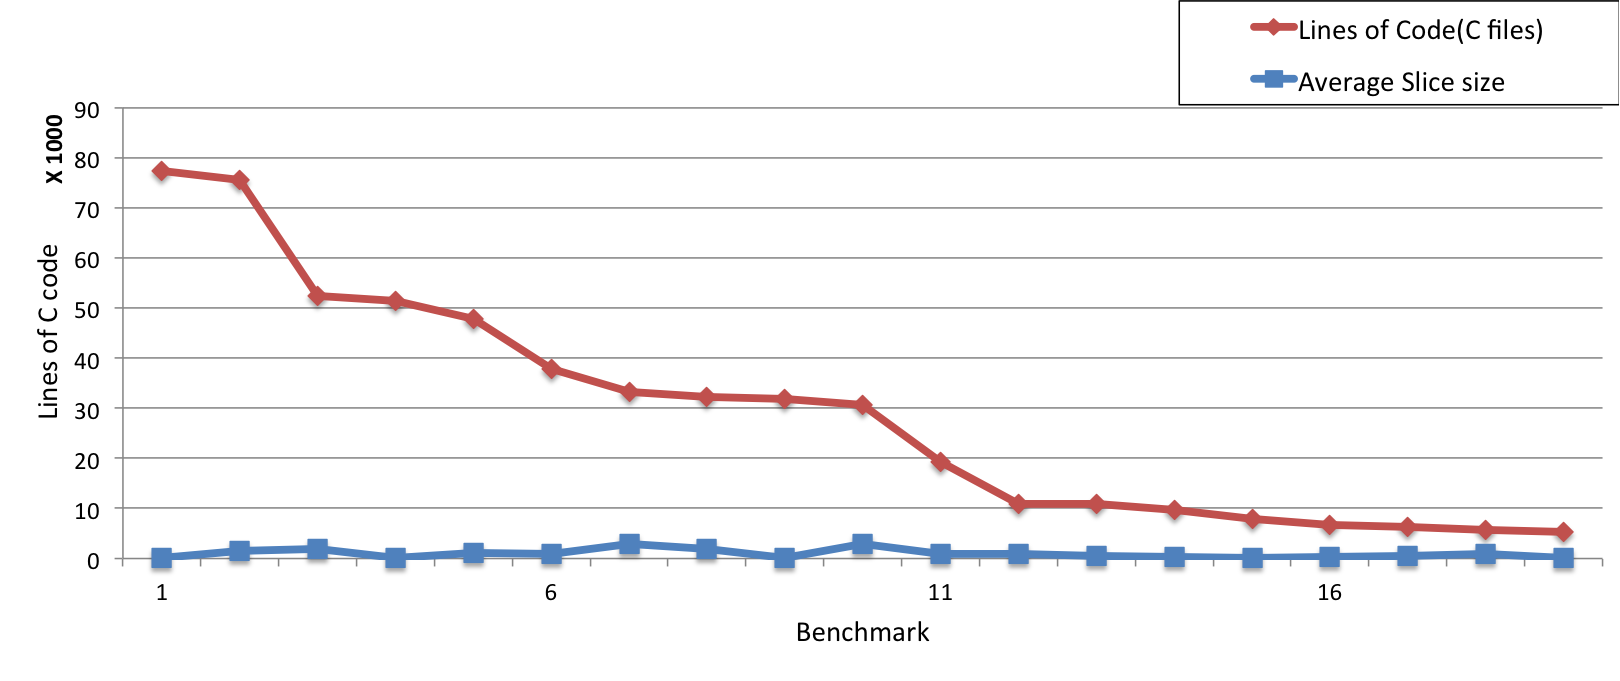
\includegraphics[width=5in]{slice-size-compare-assert.png} \\[\abovecaptionskip]
    \small (b) Assertions
  \end{tabular}
  
  \caption{Slice Size Compared to Lines of Code}\label{slice size comparison}
\end{figure}

Based on our experiment, we define the size of a slice as the number of statements in the data slice, plus the statements from the full slice that affect the value of variables in the data slice. Figure 4 compares the average size of slices with the lines of C code for each benchmark. It can seen that slice size is only a small fraction of the total lines of code. We can zoom into Figure 4 to consider only the slice size. Figure 5 shows that  more than $50\%$ benchmarks have average slice size less than 500 lines of code. Further analysis reveals that more than $80\%$ benchmarks have an average slice size less than $10\%$ of the total lines of C code in the benchmark(shown in Figure 6).\\

 
 \begin{figure}[H]
  \centering
  \begin{tabular}{@{}c@{}}
   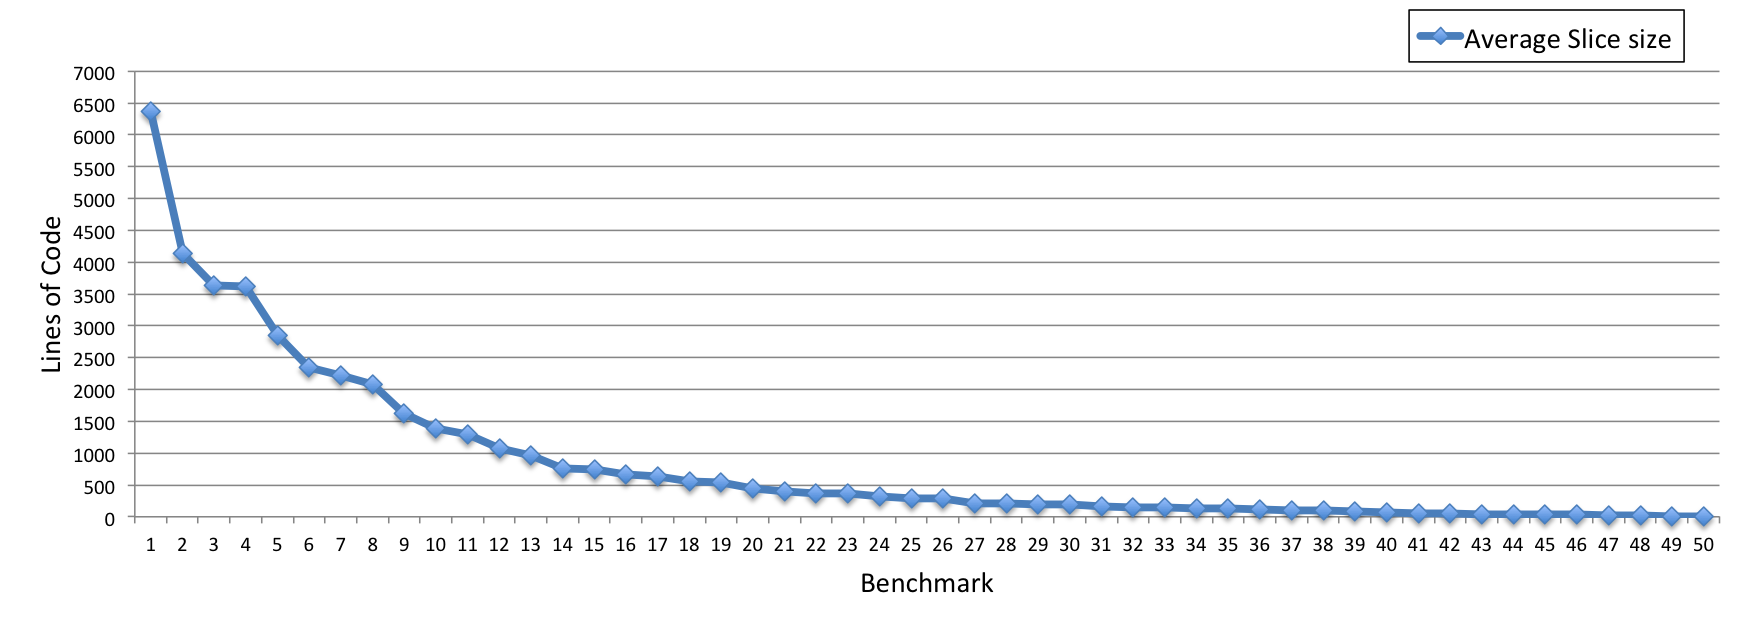
\includegraphics[width=5in]{slice-size-dec.png} \\[\abovecaptionskip]
    \small (a) Random Statements
  \end{tabular}

  \vspace{\floatsep}

  \begin{tabular}{@{}c@{}}
    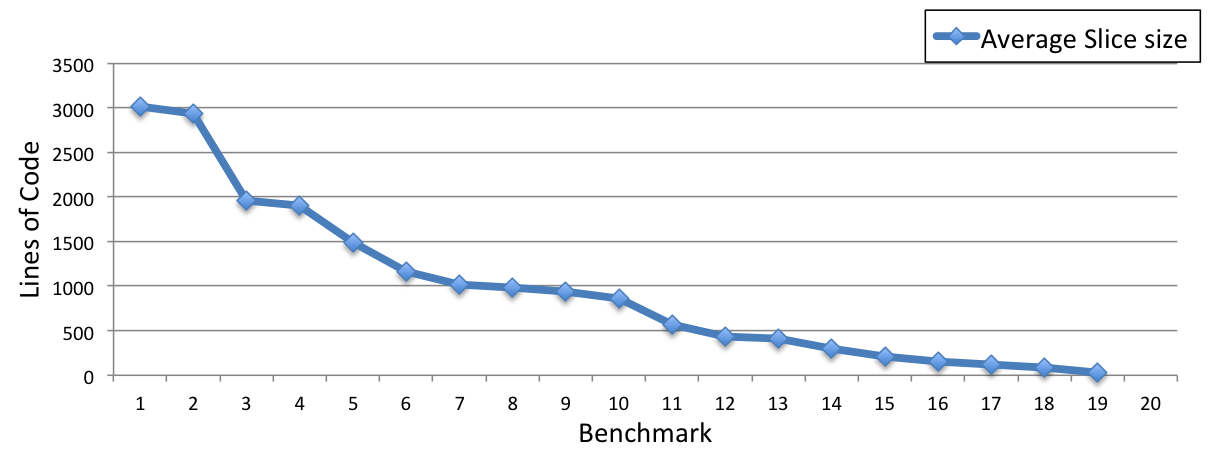
\includegraphics[width=5in]{slice-size-dec-assert.png} \\[\abovecaptionskip]
    \small (b) Assertions
  \end{tabular}
  
  \caption{Slice Size}\label{slice size distribution}
\end{figure}
 
  \begin{figure}[H]
  \centering
  \begin{tabular}{@{}c@{}}
   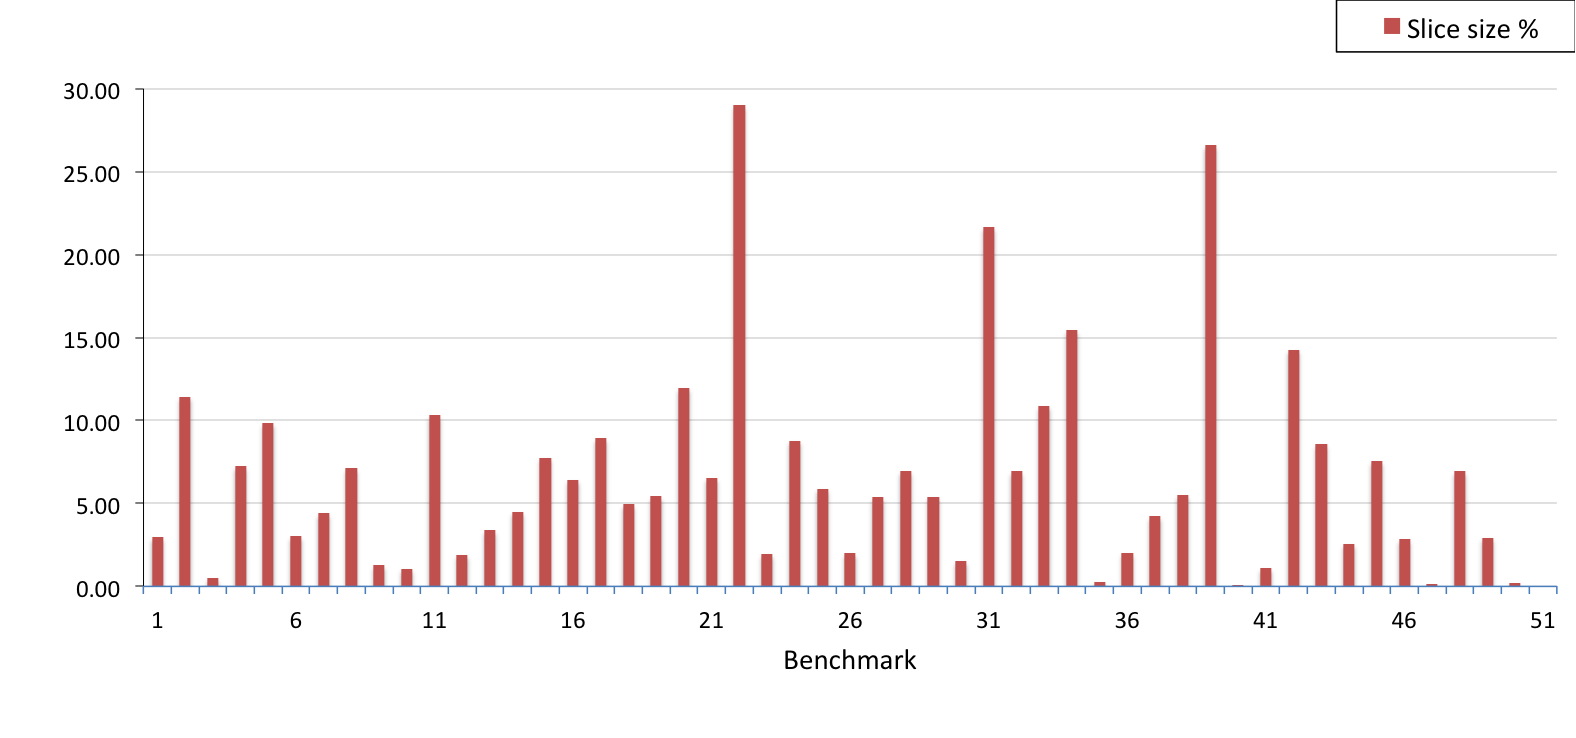
\includegraphics[width=5in]{slice-size-percent.png} \\[\abovecaptionskip]
    \small (a) Random Statements
  \end{tabular}

  \vspace{\floatsep}

  \begin{tabular}{@{}c@{}}
    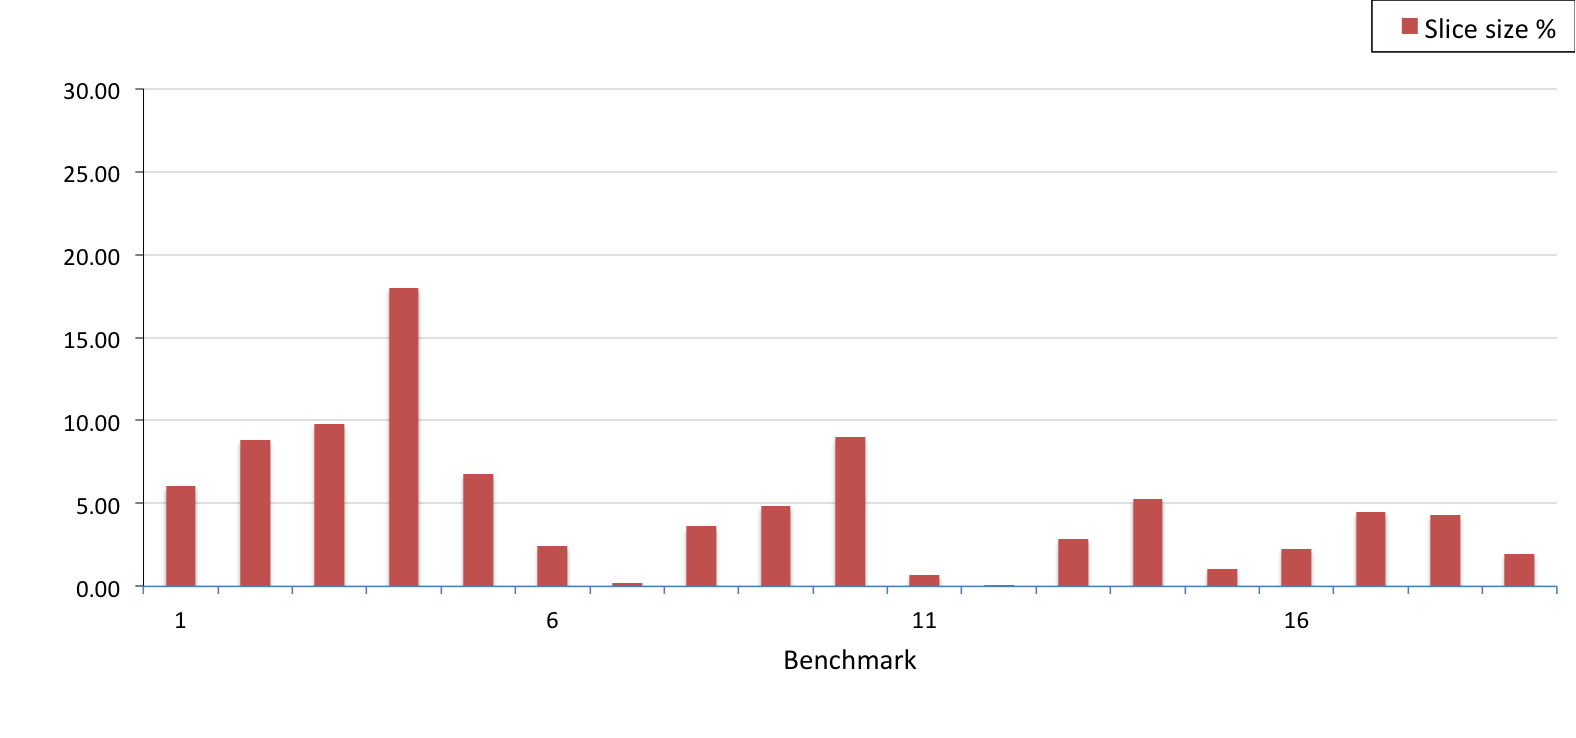
\includegraphics[width=5in]{slice-size-percent-assert.png} \\[\abovecaptionskip]
    \small (b) Assertions
  \end{tabular}
  
  \caption{Slice Size as Percentage of LOC}
  \label{slice size comparison}
\end{figure}


\begin{figure}[H]
     \centering
     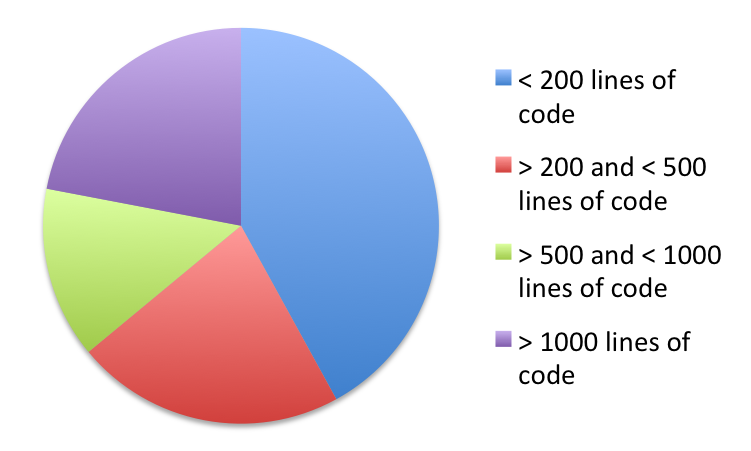
\includegraphics[width=3in]{slice-size-distribution.png}
     \caption{Slice Size Distribution - }
     \label{slice size distribution Pie}
 \end{figure}
 
 
A distribution of average slice size is shown in Figure 7. We found that a majority of benchmarks ( more than $40\%$ ) have an average slice size less than 200 lines of code. Considering the fact that a slice can include call sites and we resolve all call sites in the data slice, we are able to support our claim that demand driven dynamic analysis can focus on small fragments. Even though certain benchmarks have an average slice size greater than 200, on comparing it with the size of the benchmark, these values are negligible and this further supports our claim.  \\

\end{document}
